\chapter{Project Plan}
% [Overview of Project Plan, including any customizations to the software process model]

\section{Requirements \& Definition}
% [Plan for requirements and definition detailed here]
\textbf{Plan for requirement 1 and 2:} The plan is to use Message Queuing Telemetry
Transport (MQTT) to allow users to enter their pin using Wifi. \newline 

\textbf{Plan for requirement 3:} a 4 x 3 matrix keypad will be used as the external keypad. This will allow the user to enter their PIN. 

\textbf{Plan for requirement 4:} an external LCD will be configured to the ESP32 to display the numbers entered by the user. 

\textbf{Plan for requirement 5:} the system will use a function that will only store the last four (4) numbers entered by the user and validate the pass code. 

\textbf{Plan for requirement 6:} the system may have a timeout timer to determine if an input was entered, if not the external LCD will enable a screensaver. 


\textbf{Plan for requirement 7:} in the program, an integer array will store the \textit{correct} pass code. A function will be used to check if the user enters the correct pass code, the deadbolt will move to the unlock position. And, if the user enters the incorrect pass code, the deadbolt moves to the lock position. 

\textbf{Plan for requirement 8:} a state machine may be implemented, if the system is in a state that does not accept a PIN, the user will be unable to enter a PIN. A function will be used to determine the state. 

\textbf{Plan for requirement 9:} the system will use a function to determine if the entered PIN is correct or incorrect. If it is incorrect, the system will use a servo motor to control move the position of the deadbolt in the lock position. 

\textbf{Plan for requirement 10:} the system will use a function to determine if the entered PIN is correct or incorrect. If it is correct, the system will use a servo motor to control move the position of the deadbolt in the unlock position. 

\textbf{Plan for requirement 11:} the system will use a function to determine if the entered PIN is correct or incorrect. When the user enters a PIN, the LCD will use a function to display a message. 

\textbf{Plan for requirement 12:} in the program, an integer array will store multiple \textit{correct} pass codes. A function will be used to check if the user enters the correct pass code, the deadbolt will move to the unlock position. And, if the user enters the incorrect pass code, the deadbolt moves to the lock position. 

\section{Development}
% [Plan for development / implementation detailed here]
The goal for development of this project is to present a working prototype upon initial release and incorporate optional requirements as time allows. Project development thus far has followed the development of documentation required for class submission. In previous weeks, different peripherals were assigned to each group member and worked on individually. During initial release, the future states of the project were discussed. Moving forward, keypad software will be updated and the different functional parts of the project will be integrated to be demonstrated upon final release.

\section{Verification}
% [Plan for verification detailed here]
The goal for verification of the system will be mostly visual. First, when using the system upon startup, the user should see a prompt on the LCD to enter a PIN code. The user should then be able to enter numbers on the mechanical keypad located on the enclosure and see the LCD update in real time with the numbers entered. The LCD should only display up to six numbers - after that, the LCD should not print any more characters until an enter button is pressed. Upon this action, the LCD should display a "correct" or "incorrect" PIN code screen, determinant upon the code the user entered. Instead of the mechanical keypad, the user should also be able to input a PIN code from a dedicated mobile application, in which the LCD should display another "correct" or "incorrect" PIN code screen specific to the remote lock/unlock feature.

\section{Maintenance}
% [Plan for maintenance (e.g., problems found by prof or during updates for next release) detailed here] 
The goal for maintenance is to have a method to communicate issues with each other and document the solution for future reference. Within GitHub, an issue tracking feature is provided that allows developers to address and monitor bugs in the code. The process for reporting an issue includes describing the bug, detailing the expected behavior, and including any necessary screenshots or images. Once the issue is fixed, it should be marked as closed and a description of the solution should be provided. Additionally, commit messages are being used to detail each change in the software, and if a new change introduces an issue, we have the ability to quickly review past versions of the code and make the appropriate modifications.

\section{Umbrella Activities}
% [Plan for project management and status tracking / meetings detailed here]
Bi-weekly team meetings have been scheduled for the life-time of the project. These meetings are hosted via zoom and average 1.5 hours in length. During these meetings, documentation is generated and high-level project development is discussed. This time is used for collaboration on items
that need discussion as well as to ensure design and implementation agreement among members. The purpose of these meetings is to complete assignments and keep all group members on the same page. 
A google drive folder was created to share assignments with the group, allowing  for real-time collaboration. For larger documents, overleaf is utilized allowing for real-time collaboration as well. A GitHub repository was also created, allowing collaboration on source code as well as logging versions of code. Documentation was generated using the tools suggested by the professor and is included in the report.

\section{Responsibilities \& Gantt Chart}

\subsection{Responsibilities}
% [Describe the responsibilities of each member, how you plan to break down the work]
The goal for distributing the workload of this project is to spread the work based on skill set and comfort level of the assignment. However, there are certain tasks that have not been seen before by the team member or require more than one person to complete, therefore there are assignments that have more than one team member assigned. The following task were assigned to the respective team members: 

\begin{enumerate}
    \item \textbf{Mobile Application Implementation}
    \begin{itemize}
        \item Brendan Coffman 
    \end{itemize}

    \item \textbf{LCD Implementation}
    \begin{itemize}
        \item Isaiah Hendrick
        \item Hector Garcia
    \end{itemize}

    \item \textbf{Servo Implementation}
    \begin{itemize}
        \item Brendan Coffman 
    \end{itemize}

    \item \textbf{Keypad Implementation}
    \begin{itemize}
        \item Wade Callahan
        \item Katherine Abernathy
    \end{itemize}

\end{enumerate}

\subsection{Gantt Chart}
To create the project's Gantt Chart, the course project assignments, due dates, and additional tasks created by the team are gathered. As the project progresses, the chart's bars are filled to showcase the tasks that have been completed. A sample Gantt Chart is displayed on figured \ref{fig:Gantt Chart}.

\begin{figure}[htb]
    \begin{center}
        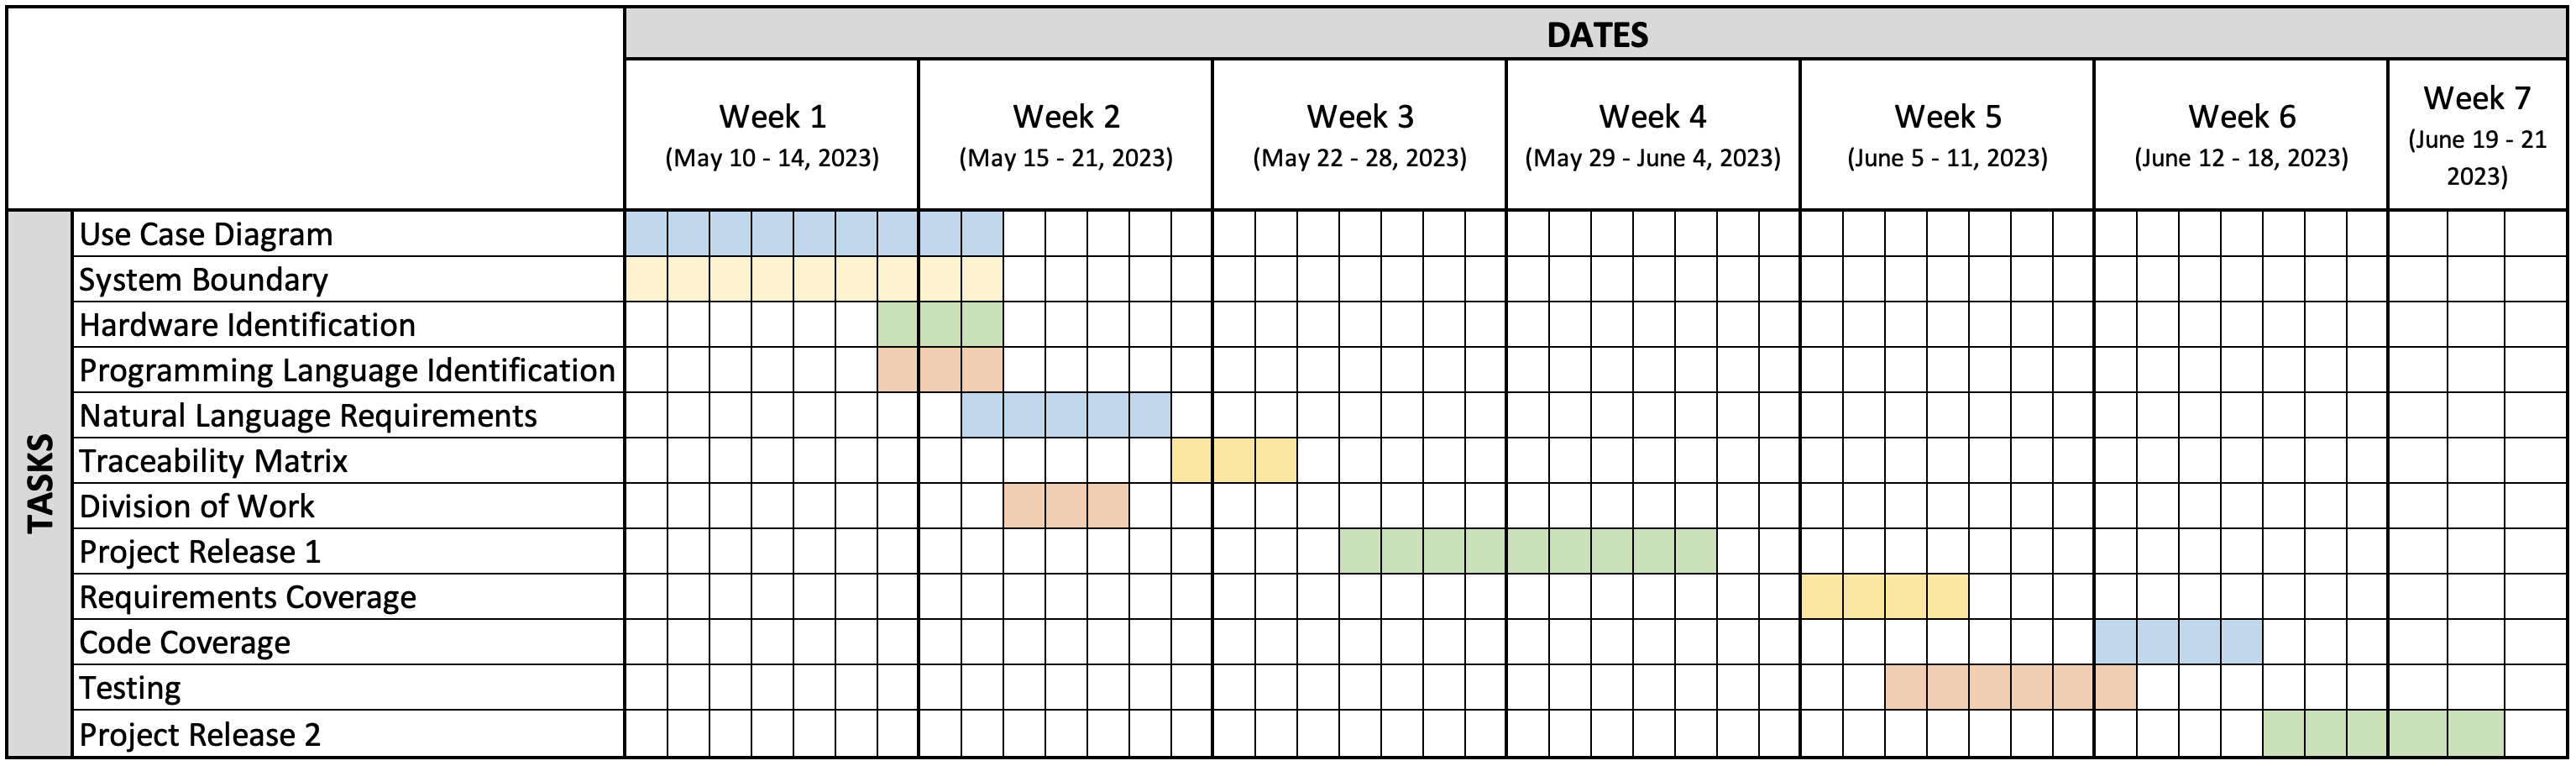
\includegraphics[width = \textwidth]{Images/CIS 350 - Project - Gantt Chart .png}
        \caption{Sample Project Gantt Chart}
        \label{fig:Gantt Chart}
    \end{center}
\end{figure}
